%%%%%%%%%%%%%%%%%%%%%%%%%%%%%%%%%%%%%%%%%
% Beamer Presentation
% LaTeX Template
% Version 1.0 (10/11/12)
%
% This template has been downloaded from:
% http://www.LaTeXTemplates.com
%
% License:
% CC BY-NC-SA 3.0 (http://creativecommons.org/licenses/by-nc-sa/3.0/)
%
%%%%%%%%%%%%%%%%%%%%%%%%%%%%%%%%%%%%%%%%%

%----------------------------------------------------------------------------------------
%	PACKAGES AND THEMES
%----------------------------------------------------------------------------------------

\documentclass{beamer}

\mode<presentation> {

% The Beamer class comes with a number of default slide themes
% which change the colors and layouts of slides. Below this is a list
% of all the themes, uncomment each in turn to see what they look like.


% \usetheme{default}
% \usetheme{AnnArbor}
% \usetheme{Antibes}
% \usetheme{Bergen}
% \usetheme{Berkeley} % neat
% \usetheme{Berlin} % nice
% \usetheme{Boadilla}
% \usetheme{CambridgeUS} %nice colors
% \usetheme{Copenhagen} % neat
% \usetheme{Darmstadt} % simple and neat
% \usetheme{Dresden} %nice and neat
% \usetheme{Frankfurt} % clean and -neat
% \usetheme{Goettingen} % clean and -neat
% \usetheme{Hannover} % neat and clean
% \usetheme{Ilmenau} % nice but dangerous layout
% \usetheme{JuanLesPins} % nice
% \usetheme{Luebeck} % clean and nice
% \usetheme{Malmoe} % same
% \usetheme{Madrid} % simple
\usetheme{Marburg} % beautiful simple and neat
% \usetheme{Montpellier} % very simple
% \usetheme{PaloAlto} % clear and nice and neat
% \usetheme{Pittsburgh}
% \usetheme{Rochester} %simple and not neat 
% \usetheme{Singapore} %meh
% \usetheme{Szeged} % a bit ugly 
% \usetheme{Warsaw} % clear and neat

% As well as themes, the Beamer class has a number of color themes
% for any slide theme. Uncomment each of these in turn to see how it
% changes the colors of your current slide theme.

% \usecolortheme{albatross}
% \usecolortheme{beaver}
% \usecolortheme{beetle}
% \usecolortheme{crane} % nice
\usecolortheme{dolphin} % very nice
% \usecolortheme{dove}
% \usecolortheme{fly}
% \usecolortheme{lily} % clean
% \usecolortheme{orchid} % clean
% \usecolortheme{rose}
% \usecolortheme{seagull}
% \usecolortheme{seahorse}
% \usecolortheme{whale} % clean
% \usecolortheme{wolverine}

% \setbeamertemplate{footline} % To remove the footer line in all slides uncomment this line
\setbeamertemplate{footline}[page number] % To replace the footer line in all slides with a simple slide count uncomment this line

\setbeamertemplate{navigation symbols}{} % To remove the navigation symbols from the bottom of all slides uncomment this line
}

\usepackage{graphicx} % Allows including images
\usepackage{booktabs} % Allows the use of \toprule, \midrule and \bottomrule in tables

%----------------------------------------------------------------------------------------
%	TITLE PAGE
%----------------------------------------------------------------------------------------

\title[Présentation]{La Physique Chimie} % The short title appears at the bottom of every slide, the full title is only on the title page

\author{A. Cercy} % Your name
\institute[] % Your institution as it will appear on the bottom of every slide, may be shorthand to save space
{
Collège Pablo Neruda
}
% \date{\today} % Date, can be changed to a custom date
\date{} % Date, can be changed to a custom date

\begin{document}

\begin{frame}
\titlepage % Print the title page as the first slide
\end{frame}

\begin{frame}
\frametitle{Plan} % Table of contents slide, comment this block out to remove it
\tableofcontents % Throughout your presentation, if you choose to use \section{} and \subsection{} commands, these will automatically be printed on this slide as an overview of your presentation
\end{frame}
%%-------------------------------------------------------------

\begin{frame}
    \frametitle{Avant de commencer}
    \centerline{Remplir, \textbf{dans le bon sens}, le plan de classe qui passe}
\end{frame}


\section{Aujourd'hui le monde est incompréhensible}
\begin{frame}
\frametitle{Aujourd'hui le monde est incompréhensible}

Quels sources d'information fiable?
\begin{itemize}
    \item fake news et infox sur internet, la télévision et la radio
    \item Les politiques
    \item Les adultes
    \item Les femmes et les hommes de science (Didier Raoult)
    \item Les enseignants?
\end{itemize}
\end{frame}

\section{Ce sera à vous de rétablir ce qui nous amené là}
    \begin{frame}
        \frametitle{Ce sera à vous de rétablir ces erreurs}

        \begin{block}{Comprendre}
        si bien le monde que vous pourrez l'expliquer aux autres
        \end{block}
    \end{frame}


\section{Le chemin vers la connaissance sera long}
\begin{frame}
\frametitle{Le chemin vers la connaissance sera long}
et je compte vous en raconter les croustillants détails.

\begin{columns}[c] % The "c" option specifies centered vertical alignment while the "t" option is used for top vertical alignment
\column{.45\textwidth} % Left column and width
    
\begin{itemize}
    \item Histoire de la logique et ses héros (Gödel).
    \item La "reine des sciences" (ou peut-on avoir une connaissance absolue sur le monde).
    \item L'informatique (car tout est sur ordinateur aujourd'hui).
    \item La science de la matière.
    \item La science des intéractions.
    \item La sociologie.
\end{itemize}
\column{.45\textwidth} % Left column and width
\begin{itemize}
    \item Alan Turing contre l'Allemagne Nazie.
    \item Gödel et l'effondrement des mathématiques.
    \item La théière de Russel.
\end{itemize}

\end{columns}
\end{frame}




\subsection{L'important c'est de trouver son chemin à soi}
\begin{frame}
\frametitle{L'important c'est de trouver son chemin à soi}
\begin{columns}[c] % The "c" option specifies centered vertical alignment while the "t" option is used for top vertical alignment

\column{.45\textwidth} % Left column and width
\textbf{Parfois}
la physique chimie ce n'est pas le plus urgent dans l'immédiat,
parfois on va mal, on est fatigué.e, on a d'autres problèmes

\column{.5\textwidth} % Right column and width
C'est tout à fait normal, c'est pour ça que c'est 
si important de se respecter les uns les autres

\end{columns}

\end{frame}

\section{We need you}
\begin{frame}
\frametitle{We need you}
\begin{figure}
    
\includegraphics[width=0.8\linewidth]{we_need_you.jpg}
\end{figure}
\end{frame}

\begin{frame}
    \frametitle{Une classe accueillante pour tous}
    \begin{itemize}
        \item Peu importe son genre (garçon ou fille)
        \item Peu importe sa sexualité
        \item Peu importe son style etc
    \end{itemize}
\end{frame}


\begin{frame}
\frametitle{M'aider à orienter mon cours}

\begin{itemize}
    \item En me disant ce qui vous intéresse 
    (et à la fin de l'année, ce qui ne vous à pas intéressé).

    La boite à suggestion
    \item En participant et vous investissant
\end{itemize}

\end{frame}

\subsection{Règles de vie de classe}
\begin{frame}
\frametitle{Discussion sur des principes importants}
\begin{itemize}
    \item que faut-il faire en classe?
    \item que faut-il ne pas faire?
    \item Pourquoi?
    \item Que fait on si quelqu'un ne respecte pas ces principes?
\end{itemize}

\begin{enumerate}
    \item Discutons en ensemble.
    \item Coller sur la deuxième page du cahier le document distribué.
\end{enumerate}
\end{frame}


\subsection{Apprenons à nous connaître}
\begin{frame}
\frametitle{Apprenons à nous connaître}
\begin{enumerate}
    \item Je distribue le questionnaire
    \item Vous le remplissez 
\end{enumerate}
\end{frame}

\subsection{La physique chimie, c'est quoi?}
    \begin{frame}
    \frametitle{La physique chimie, c'est quoi?}
    \begin{figure}
        
\includegraphics[width=0.8\linewidth]{atome.jpg}
    \end{figure}
    \end{frame}

    \begin{frame}
        \frametitle{ça?}
        
        \begin{figure}
            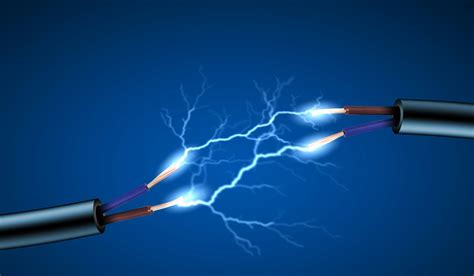
\includegraphics[width=0.8\linewidth]{electricite.jpg}
    \end{figure}
    \end{frame}

    \begin{frame}
        \frametitle{peut être ça?}
        
        \begin{figure}
            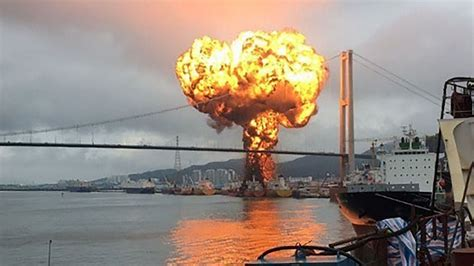
\includegraphics[width=0.8\linewidth]{explosion.jpg}
    \end{figure}
    \end{frame}

    \begin{frame}
        \frametitle{ou bien ça?}
        
        \begin{figure}
            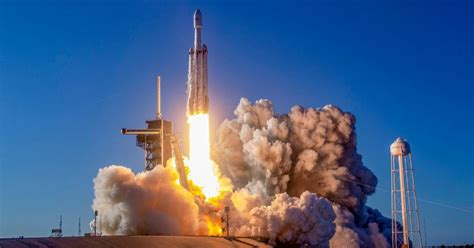
\includegraphics[width=0.8\linewidth]{fusee.jpg}
    \end{figure}
    \end{frame}

    \begin{frame}
        \frametitle{ou un peu tout ça à la fois...}
        
        \begin{figure}
            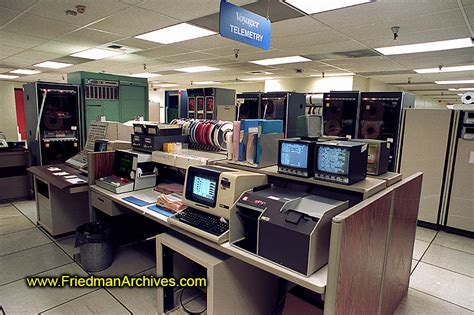
\includegraphics[width=0.8\linewidth]{nasa_computer.jpg}
    \end{figure}
    \end{frame}
    

    \begin{frame}
        \begin{center}
            Correction du questionnaire
        \end{center}
    \end{frame}

    \begin{frame}
        \begin{center}
            Brainstorming sur qu'est-ce que la physique chimie et à quoi ça sert
        \end{center}
    \end{frame}


    \begin{frame}
        \frametitle{Les devoirs pour la prochaine fois}
        \begin{enumerate}
            \item Faire la page de garde de son cahier ou porte-vues
            (nom, prénom, matière, année, nom de l'enseignant.e)
            \item Signer le document : 'bien fonctionner en physique chimie' 
        \end{enumerate}
    \end{frame}



%------------------------------------------------

\begin{frame}
\Huge{\centerline{Fin}}
\end{frame}

%----------------------------------------------------------------------------------------

\end{document} 